% vim:set ts=2 sw=2 noet:
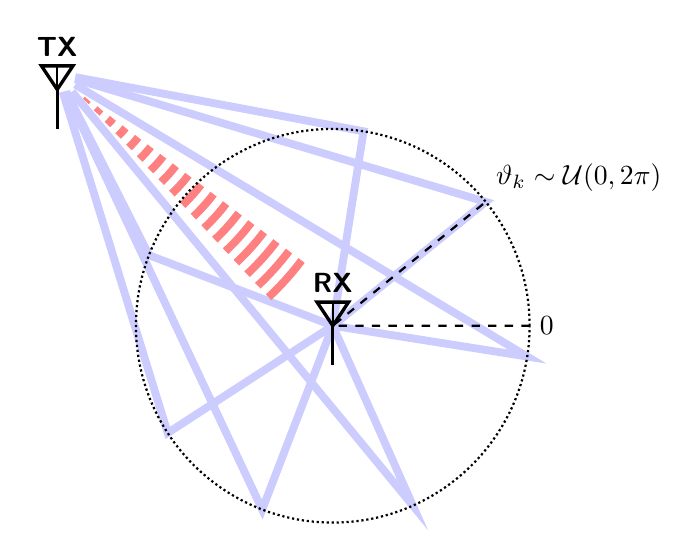
\begin{tikzpicture}[
			antenna/.pic = {
				\draw[very thick] (0,0) -- ++(2mm, 3mm) -- ++(-4mm,0) -- cycle;
				\draw[very thick] (0,0) -- ++(0,-5mm) coordinate (-mast) {};
				\draw[thick] (0,0) -- ++(0,3mm);
				\node[inner sep = 0pt, outer sep = 6pt] (-center) at (0,2mm) {};
			},
	]

	\coordinate (X) at (-3.5,3);

	% antennas
	\draw (X) pic (T) {antenna} node[above = 3mm] {\sffamily\bfseries TX};

	% rays
	\foreach \i [count=\j] in {-2.2,-0.3,1.3,2.7,5.3,7.1,8.3}{
		\draw[blue!20, line width = 1mm]
			(T-center) -- ({30 * \i}:25mm) coordinate (p\j) -- (0,0);
	};

	% angle
	\draw[dashed, thick] (25mm, 0) node[right] {0}
		-- (0,0) -- (p3) node[above right] {\(\vartheta_k \sim \mathcal{U}(0,2\pi)\)};

	% LOS
	\draw[line width = 1mm, red!50,
		decorate, decoration = {
			expanding waves, angle = 5, segment length = 2mm
		}
	] (T-center) -- (-5mm, 5mm);

	% ring und RX antenna
	\draw (0,0) pic (R) {antenna} node[above = 3mm] {\sffamily\bfseries RX};
	\draw[thick, densely dotted] circle (25mm);
	

\end{tikzpicture}
